\documentclass[a4paper, 12pt]{report}

\usepackage{lmodern} % Police standard sous LaTeX : Latin
\usepackage[english]{babel} % Pour la langue anglaise
\usepackage[utf8]{inputenc} % Pour l'UTF-8
\usepackage[T1]{fontenc} % Pour les césures des caractères
\usepackage{graphicx}
\usepackage{subfig}
\usepackage{ragged2e}
\justifying

\renewcommand{\thesection}{\Alph{section}}

\title{Model of the spread of a disease in a population of mobile agents}
\author{NIDDAM Benjamin}
\date{\today}

\begin{document}
\begin{titlepage}
	\maketitle
\end{titlepage}

\newpage

\tableofcontents

\newpage
\section{Introduction}

After the discovery of a new disease, we seek to study its behavior on a population of mobile agents.
Secondly, we will study different strategies to contain its spread. So we want, at the end,
know the most effective means (s) to prevent the disease from spreading in the population.

\section{Model presentation}
\subsection{Variables definition}

The first step is to define the different parameters of the simulation. We will have:
\begin{itemize}
	\item a simulation duration,
	\item a number of agents,
	\item a number of agents contaminated at time zero,
	\item a degree of confinement of the population,
	\item a degree of respect for barrier gestures.
\end{itemize}

\subsection{Agents presentation}

Our agents are represented by circles of coordinates (x, y) and radius (r). They have a Boolean contamination state, a contamination probability (p), a Boolean healing state and
a boolean impunity state. These states are modified by interactions between agents and defined durations which seek to be closest to reality. The agents evolve in a square world
of dimension (w, h) and are placed randomly in this world with a speed (vx, vy), also random.

\subsection{interactions definition}

There is only one type of interaction between our agents. It is the contagion interaction. When an agent is contaminated, it can infect other agents but can no longer be
contaminated. For a healthy agent to become contaminated, it must meet certain conditions. It must be a defined contamination radius (ir). He must be healthy, not be immune
and not be vaccinated.

\begin{figure}[h]
	\centering
	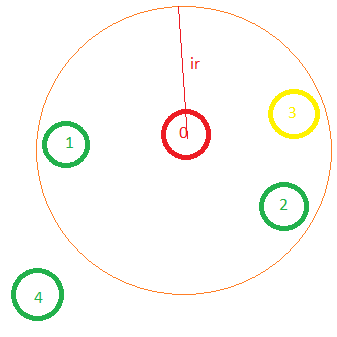
\includegraphics[width=0.5\textwidth]{./Interactions.png}
	\caption{Interaction between agents}
\end{figure}

In this exemple, only the agents in the infection radius (ir) can be infected, only if their not immune(yellow) or infected(red).

% \newpage
\newpage


\section{Experiments, results and limitations}
\subsection{initial state}

In all of our simulations, we used a number of agents fixed to 1000, a number of contaminated agents fixed to 1 and 100 and a 3.5\% contamination degree.
Before starting the tests to contain the disease, we simulated the the evolution of the infecteds agents without any intervention.
Here are the results:

\begin{figure}[h]

	\centering
	\subfloat[\centering 1 infected agent at t0]{{\includegraphics[width=6cm]{../Courbes/1000_agents_1_contaminé_5_ans/Natural_immunity_only.png} }}
	\qquad
	\subfloat[\centering 100 infecteds agents at t0]{{\includegraphics[width=6cm]{../Courbes/1000_agents_100_contaminé_5_ans/Natural_immunity_only.png} }}
	\centering
	\caption{Graphic representations of the evolution of the condition of the population as a function of time}

\end{figure}

\newpage

The infecteds evolution is represented by a succesion of contamination and healing waves that spread until the end of the simulation. These waves are due to the fact that our agents
gain a temporary immunity after each healing.

\vspace{0.8cm}

There are various expériences that we have done trying to contain or eradicate the disease. For each of these experiments, we simulated it four times with the same initial conditions
and used the average of the results as a representative result to reduce the uncertainty due to randomness.


\subsection{Confinement}

As a first experiment we decided to confine the population. To do this we divide the
values of vx and vy by two, then by three and finally by five. Which brings us back to three tests that we
call respectively "light confinement", "medium confinement" and "strict confinement" in relation to their
limitation rate. This rate will reduce the possibility of moving for the agents until almost immobility
when the rate is near to five. This therefore leads to a reduction in interactions between agents which should
limit the spread of the disease. We want to know if this reduction is sufficient to eradicate the disease. And
if so, what rate should be set up and sure how long. We therefore carried out the simulations
following:

\begin{figure}[h]
	\centering
	\subfloat[\centering Light confinement]{{\includegraphics[width=6cm]{../Courbes/1000_agents_1_contaminé_5_ans/Light_confinement.png} }}
	\qquad
	\subfloat[\centering Basic confinement]{{\includegraphics[width=6cm]{../Courbes/1000_agents_1_contaminé_5_ans/Partial_confinement.png} }}
\end{figure}
\begin{figure}[h]
	\centering
	\subfloat[\centering Heavy confinement]{{\includegraphics[width=6cm]{../Courbes/1000_agents_1_contaminé_5_ans/Strict_confinement.png} }}
	\qquad
	\caption{Graphical representations of the evolution of the state \\ of the population as a function of the confinement rate}
\end{figure}
\newpage

The graphs above represent the evolution of the state of the agents during the simulation according to the rate of confinement.
It is observed that the method of confinement is a very effective way of slowing the movement of the disease within the population. We can clearly see it
on the graphs of light and medium confinement. Indeed, the initial contamination peak is much less important than the one of the simulation without restrictions.
Finally, based on the strict confinement curve, it is confirmed that this method, despite a very significant degree of limitations, is not sufficient to eradicate the disease.
We can therefore consider combining it with another method. But before that, we tested whether to set up a confinement of the population while the epidemic has already spread.
We obtained the following results:

\begin{figure}[!h]
	\centering
	\subfloat[\centering Light confinement]{{\includegraphics[width=6cm]{../Courbes/1000_agents_100_contaminé_5_ans/Light_confinement.png} }}
	\qquad
	\subfloat[\centering Basic confinement]{{\includegraphics[width=6cm]{../Courbes/1000_agents_100_contaminé_5_ans/Partial_confinement.png} }}
\end{figure}
\begin{figure}[!h]
	\centering
	\subfloat[\centering Heavy confinement]{{\includegraphics[width=6cm]{../Courbes/1000_agents_100_contaminé_5_ans/Strict_confinement.png} }}
	\qquad
	\caption{Graphical representations of the evolution of the state \\ of the population as a function of the confinement rate}

\end{figure}

\newpage

Thanks to this second set of simulations, it appears that when confinement is decreed from the first cases, we notice that there is no peak of contamination whatever the rate of confinement.
In comparison with simulations where confinement begins with 10\% of the infected population, in which confinement only allows
to reduce the first peak of contamination. In the long term, containment, whatever its intensity, stabilizes the number of daily infected.


\subsection{Respect for barrier gestures}

Secondly, we decided to implement a respect for barrier gestures. This method seeks to reduce the probability that a contaminated agent transmite the disease to another agent
when they meet. To do this, we have set up three intensities: "Basics barrier gestures", "Mediums barrier gestures" and "Heavys barrier gestures" which reduce by two, three and five
the probability of infection. In this case, we want to know to what level the barrier gestures can slow down the disease.

\begin{figure}[h]
	\centering
	\subfloat[\centering Basics barrier gestures]{{\includegraphics[width=6cm]{../Courbes/1000_agents_1_contaminé_5_ans/Basics_barrier_gestures.png} }}
	\qquad
	\subfloat[\centering Mediums barrier gestures]{{\includegraphics[width=6cm]{../Courbes/1000_agents_1_contaminé_5_ans/Mediums_barrier_gestures.png} }}
	\centering
	\subfloat[\centering Heavys barrier gestures]{{\includegraphics[width=6cm]{../Courbes/1000_agents_1_contaminé_5_ans/Heavys_barrier_gestures.png} }}
	\qquad
	\caption{Graphic representations of the evolution of the state \\ of the population according to the rate of barrier gestures}

\end{figure}

\newpage

Here, we represent the evolution of the state of the agents over time according to the degree of respect of the population for the barrier gestures.
We can clearly see that the barrier gestures are very effective in reducing the transmission of the disease even if the agents do not follow them strictly as shown in the graph.
"basic barrier gestures".
Thanks to the curves, it is clear that barrier gestures are a very good
convenient to reduce disease transmission. In addition, as shown in the graph "strict barrier gestures", if respected seriously and from the first days, an epidemic can easily
be avoided. But we can also wonder if this method would also be useful, if implemented while the epidemic is already underway. Here are the results obtained for this case:

\begin{figure}[h]
	\centering
	\subfloat[\centering Light barrier gestures]{{\includegraphics[width=6cm]{../Courbes/1000_agents_100_contaminé_5_ans/Basics_barrier_gestures.png} }}
	\qquad
	\subfloat[\centering Basic barrier gestures]{{\includegraphics[width=6cm]{../Courbes/1000_agents_100_contaminé_5_ans/Mediums_barrier_gestures.png} }}
	\centering
	\subfloat[\centering Heavy barrier gestures]{{\includegraphics[width=6cm]{../Courbes/1000_agents_100_contaminé_5_ans/Heavys_barrier_gestures.png} }}
	\qquad
	\caption{Graphical representations of the evolution of the state \\ of the population as a function of the rate of barrier gestures}

\end{figure}

\newpage

In the present case, the development of the disease is attenuated by the barrier gestures. However, as for the previous experience, except when barrier gestures are strongly respected,
the epidemic is not avoided.

\newpage

\subsection{Vaccination}

We then set up a vaccination cycle. In fact, in the simulation, each day, we vaccinate a number of agents defined in advance.The vaccine gives a longer immunity than that obtained
naturally. In the midst of this experience, we were able to test several things. At first, the agents perform only one vaccination which immunizes them for a while but ends
by catching the disease at the end of their vaccination period.

\begin{figure}[h]
	\centering
	\subfloat[\centering 1 dayly vaccination]{{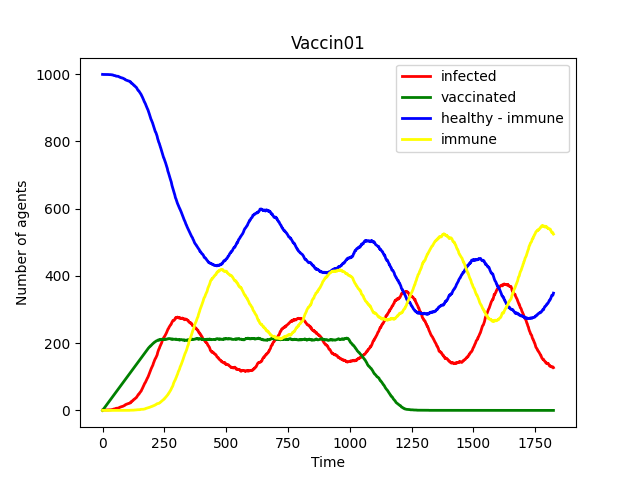
\includegraphics[width=6cm]{../Courbes/1000_agents_1_contaminé_5_ans/Vaccin01.png} }}
	\qquad
	\subfloat[\centering 3 dayly vaccination]{{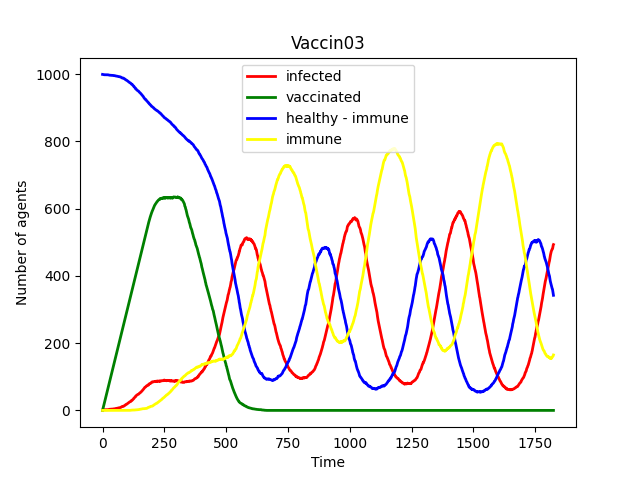
\includegraphics[width=6cm]{../Courbes/1000_agents_1_contaminé_5_ans/Vaccin03.png} }}
	\centering
	\subfloat[\centering 4 dayly vaccination]{{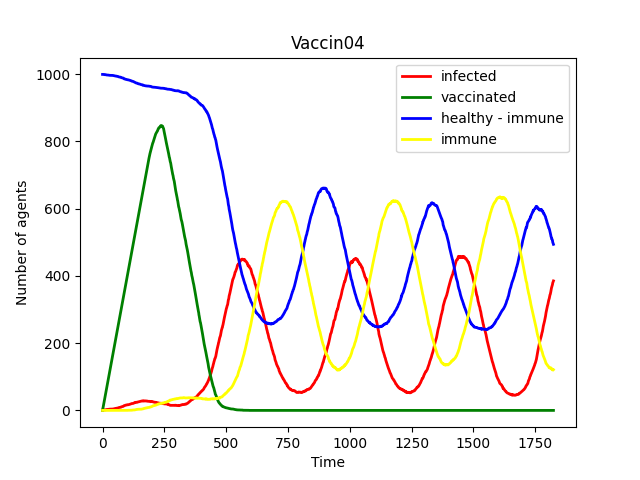
\includegraphics[width=6cm]{../Courbes/1000_agents_1_contaminé_5_ans/Vaccin04.png} }}
	\qquad
	\caption{Graphical representations of the evolution of the state \\ of the population according to the number of new vaccinated per day}

\end{figure}

These graphs represent the evolution of the state of the population as a function of time for a number of people who are vaccinated each day.
It is observed that having part of the population vaccinated is a good practice to reduce the transmission of the disease. Indeed, the peak of vaccination] makes it possible to
greatly delayed the initial contamination peak.

\newpage

In addition, we can see that the number of people who get vaccinated every day is an important factor to delay the explosion of the epidemic.

Subsequently, we implemented the vaccine boosters. We revaccinate agents when their vaccine no longer works. We therefore look at the minimum threshold of people to be vaccinated per day
for the disease to be eradicated.

\begin{figure}[h]
	\centering
	\subfloat[\centering 1 dayly vaccination]{{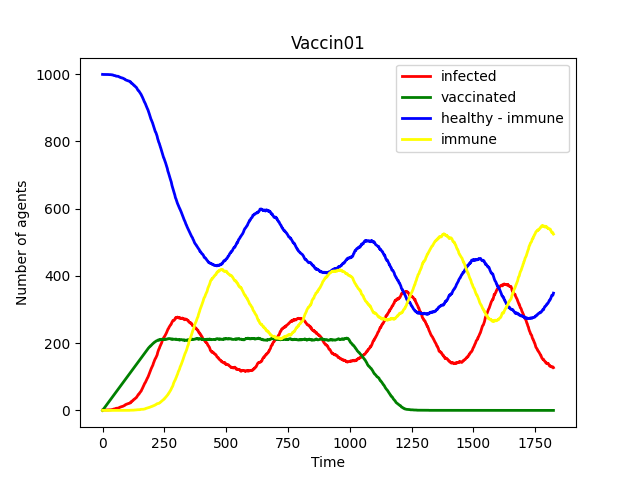
\includegraphics[width=6cm]{../Courbes/1000_agents_1_contaminé_5_ans/Vaccin01.png} }}
	\qquad
	\subfloat[\centering 3 dayly vaccination]{{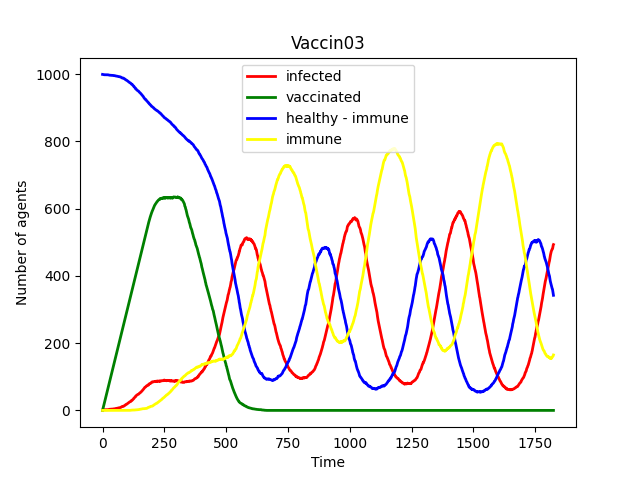
\includegraphics[width=6cm]{../Courbes/1000_agents_1_contaminé_5_ans/Vaccin03.png} }}
	\centering
	\subfloat[\centering 4 dayly vaccination]{{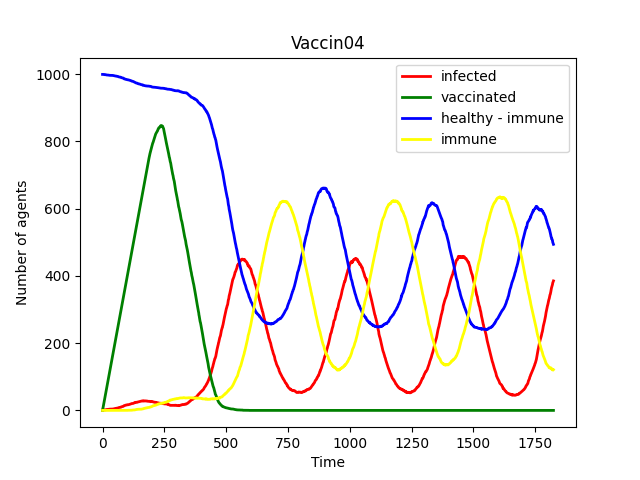
\includegraphics[width=6cm]{../Courbes/1000_agents_1_contaminé_5_ans/Vaccin04.png} }}
	\qquad
	\caption{Graphical representations of the evolution of the state \\ of the population according to the number of new vaccinated per day}

\end{figure}

These graphs showing the evolution of the state of the population as a function of time for a number of people who are dayly vaccinated clearly show that
getting vaccinated regularly makes it very easy to eradicate the disease. In fact, it is observed that from three additional people vaccinated per day, the disease does not exceed 15% of infected.
and that is enough to vaccinate four people per day to eradicate the disease after two years for a population of 1000 agents.

\newpage

We repeated the "vaccine" experiment, but with a number of agents contaminated at 100 at t0 to simulate an epidemic in progress.

\begin{figure}[h]
	\centering
	\subfloat[\centering 1 dayly vaccination]{{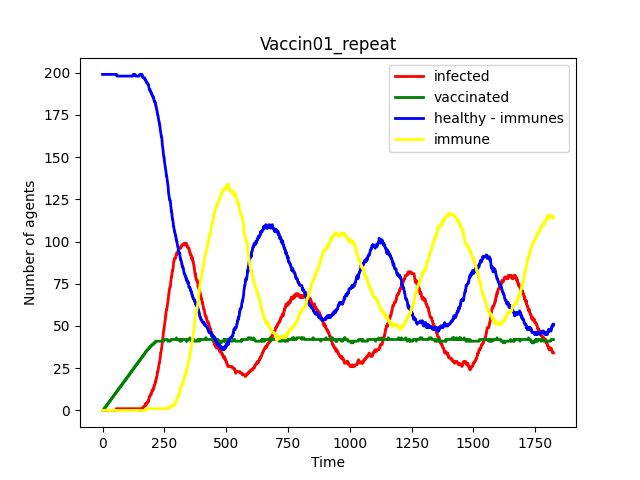
\includegraphics[width=6cm]{../Courbes/1000_agents_100_contaminé_5_ans/Vaccin01_repeat.png} }}
	\qquad
	\subfloat[\centering 3 dayly vaccination]{{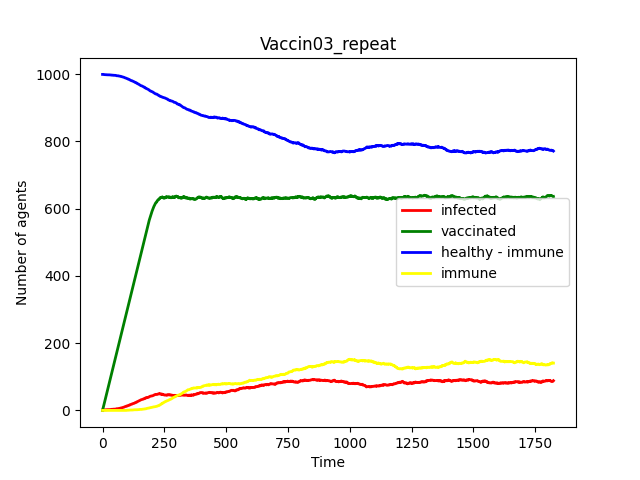
\includegraphics[width=6cm]{../Courbes/1000_agents_100_contaminé_5_ans/Vaccin03_repeat.png} }}
	\centering
	\subfloat[\centering 4 dayly vaccination]{{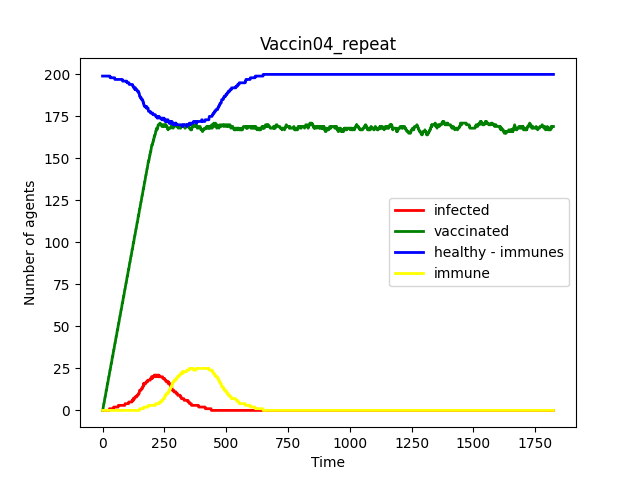
\includegraphics[width=6cm]{../Courbes/1000_agents_100_contaminé_5_ans/Vaccin04_repeat.png} }}
	\qquad
	\caption{Graphical representations of the evolution of the state \\ of the population according to the number of new vaccinated per day}

\end{figure}

We come to the same conclusions as in the previous experience, the vaccine is the best practice to eradicate the disease and it is necessary to vaccinate at least three people per day to
that the results are really significant.

\newpage

\subsection{combination of methods}

Finally, after presenting the different ways of hindering the spread of a disease within a population, we decided to test different combinations of methods.
We therefore present two of them:

\begin{itemize}
	\item Light confinement and medium barrier gestures
	\item Mediums barrier gestures and vaccin 3 people per day with vaccin booster
\end{itemize}

\begin{figure}[h]
	\subfloat[\centering Light confinement and medium barrier gestures]{{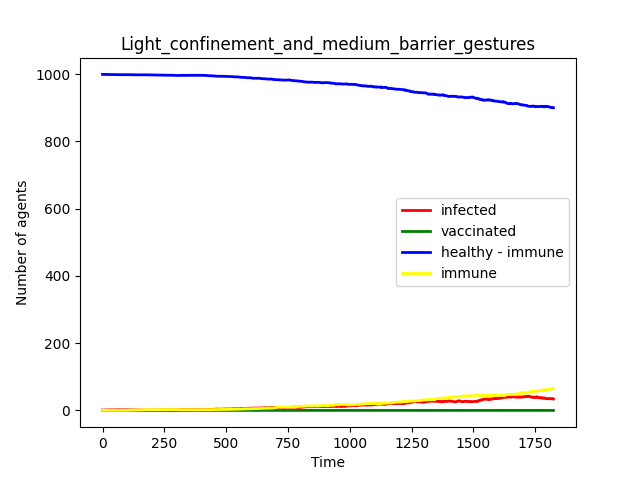
\includegraphics[width=6cm]{../Courbes/1000_agents_1_contaminé_5_ans/Light_confinement_and_medium_barrier_gestures.png} }}
	\subfloat[\centering Mediums barrier gestures and vaccin 3 people per day with vaccin booster]{{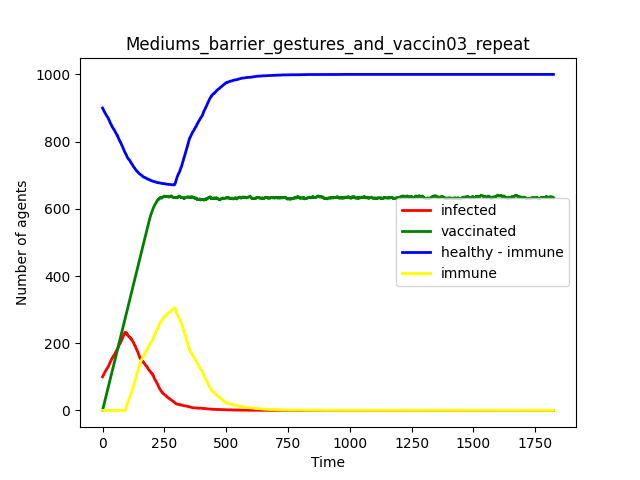
\includegraphics[width=6cm]{../Courbes/1000_agents_1_contaminé_5_ans/Mediums_barrier_gestures_and_vaccin03_repeat.png} }}
	\caption{Graphical representations of the evolution of the state \\ of the population according to the combination of methods}
\end{figure}

Since the methods combined here have proved their worth individually, we have therefore been able to see that the results are significant. However, for light confinement and medium barrier gestures, we see
that the disease is more difficult to eradicate. Since these two methods are used more to slow the spread than to eradicate it, we observe that the disease is progressing all the same.
While Mediums barrier gestures and vaccine 3 people per day with vaccine booster does not even allow the disease to progress.

\newpage

\section{Conclusion}

After this battery of tests, we are able to define the most effective way to counter this new disease. First of all, if the latter is noticed early enough,
light confinement with a population that pays attention to basic barrier gestures, would greatly slow down its spread while awaiting the development of a vaccine that would eradicate it.

\end{document}

